
\documentclass[12pt]{article}
\usepackage[utf8]{inputenc}
\usepackage{graphicx}
\usepackage{amsmath}
\usepackage{booktabs}
\usepackage{caption}
\usepackage{subcaption}
\usepackage{geometry}
\usepackage{hyperref}
\usepackage{float}
\usepackage{enumitem}
\usepackage{xcolor}

% Page geometry
\geometry{a4paper, margin=1in}

% Hyperref settings
\hypersetup{
    colorlinks=true,
    linkcolor=blue,
    filecolor=magenta,
    urlcolor=cyan
}

% Custom commands
\newcommand{\datasetname}[1]{\textbf{#1}}
\newcommand{\paramname}[1]{\texttt{#1}}

% Title page
\begin{document}
\begin{titlepage}
    \centering
    \vspace*{2cm}

    % Logo
    
\includegraphics[width=0.4\textwidth]{scagentic_logo.png}
    \vspace{1cm}

    % Title
    \Huge\textbf{Single-Cell RNA-seq Analysis Report}
    \vspace{1cm}

    % Study information
    \Large\textbf{Single-cell RNA-seq analysis of GSM7770556}
    \vspace{0.5cm}

    % GEO accession
    \Large\textbf{GEO Accession: GSM7770556}
    \vspace{0.5cm}

    % Species and tissue
    \Large\textbf{Species: Homo sapiens}
    \vspace{0.5cm}
    \Large\textbf{Tissue: Not specified}
    \vspace{1cm}

    % Date
    \large\today
\end{titlepage}

% Table of contents
\tableofcontents
\newpage

% Study information
\section{Study Information}
\begin{itemize}
    \item \textbf{GEO Accession:} GSM7770556
    \item \textbf{Species:} Homo sapiens
    \item \textbf{Tissue:} Not specified
    \item \textbf{Analysis Date:} March 30, 2025
\end{itemize}

% Analysis parameters
\section{Analysis Parameters}
\begin{table}[H]
    \centering
    \begin{tabular}{ll}
        \toprule
        \textbf{Parameter} & \textbf{Value} \\
        \midrule
        Min Genes & 200 \\
        Min Cells & 3 \\
        Max Percent Mt & 20 \\
        N Top Genes & 2000 \\
        N Pcs & 50 \\
        Resolution & 0.5 \\

        \bottomrule
    \end{tabular}
    \caption{Analysis parameters used in preprocessing}
    \label{tab:parameters}
\end{table}

% Results
\section{{Results}}

    \begin{figure}[H]
        \centering
        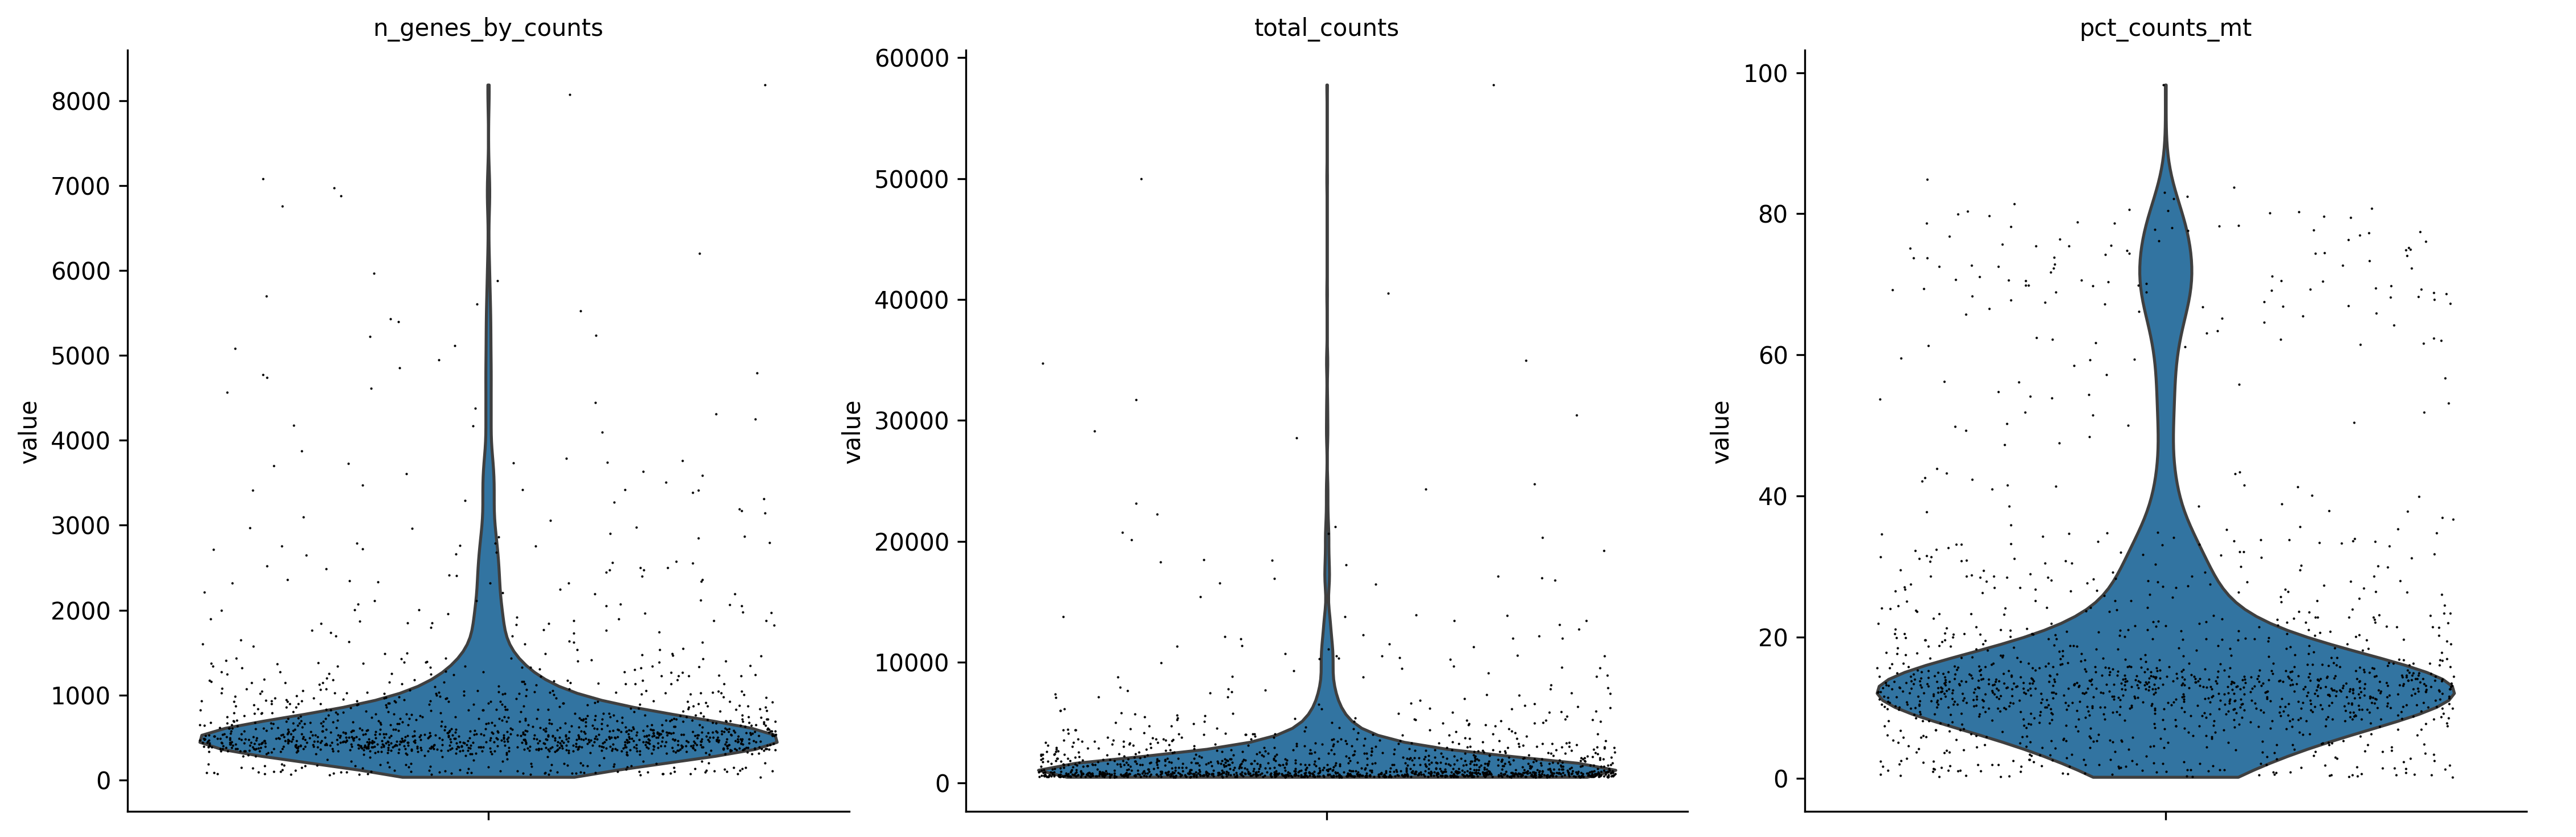
\includegraphics[width=0.8\textwidth]{qc_distributions.png}
        \caption{Qc Distributions}
        \label{fig:qc_distributions}
    \end{figure}
    \newpage

    \begin{figure}[H]
        \centering
        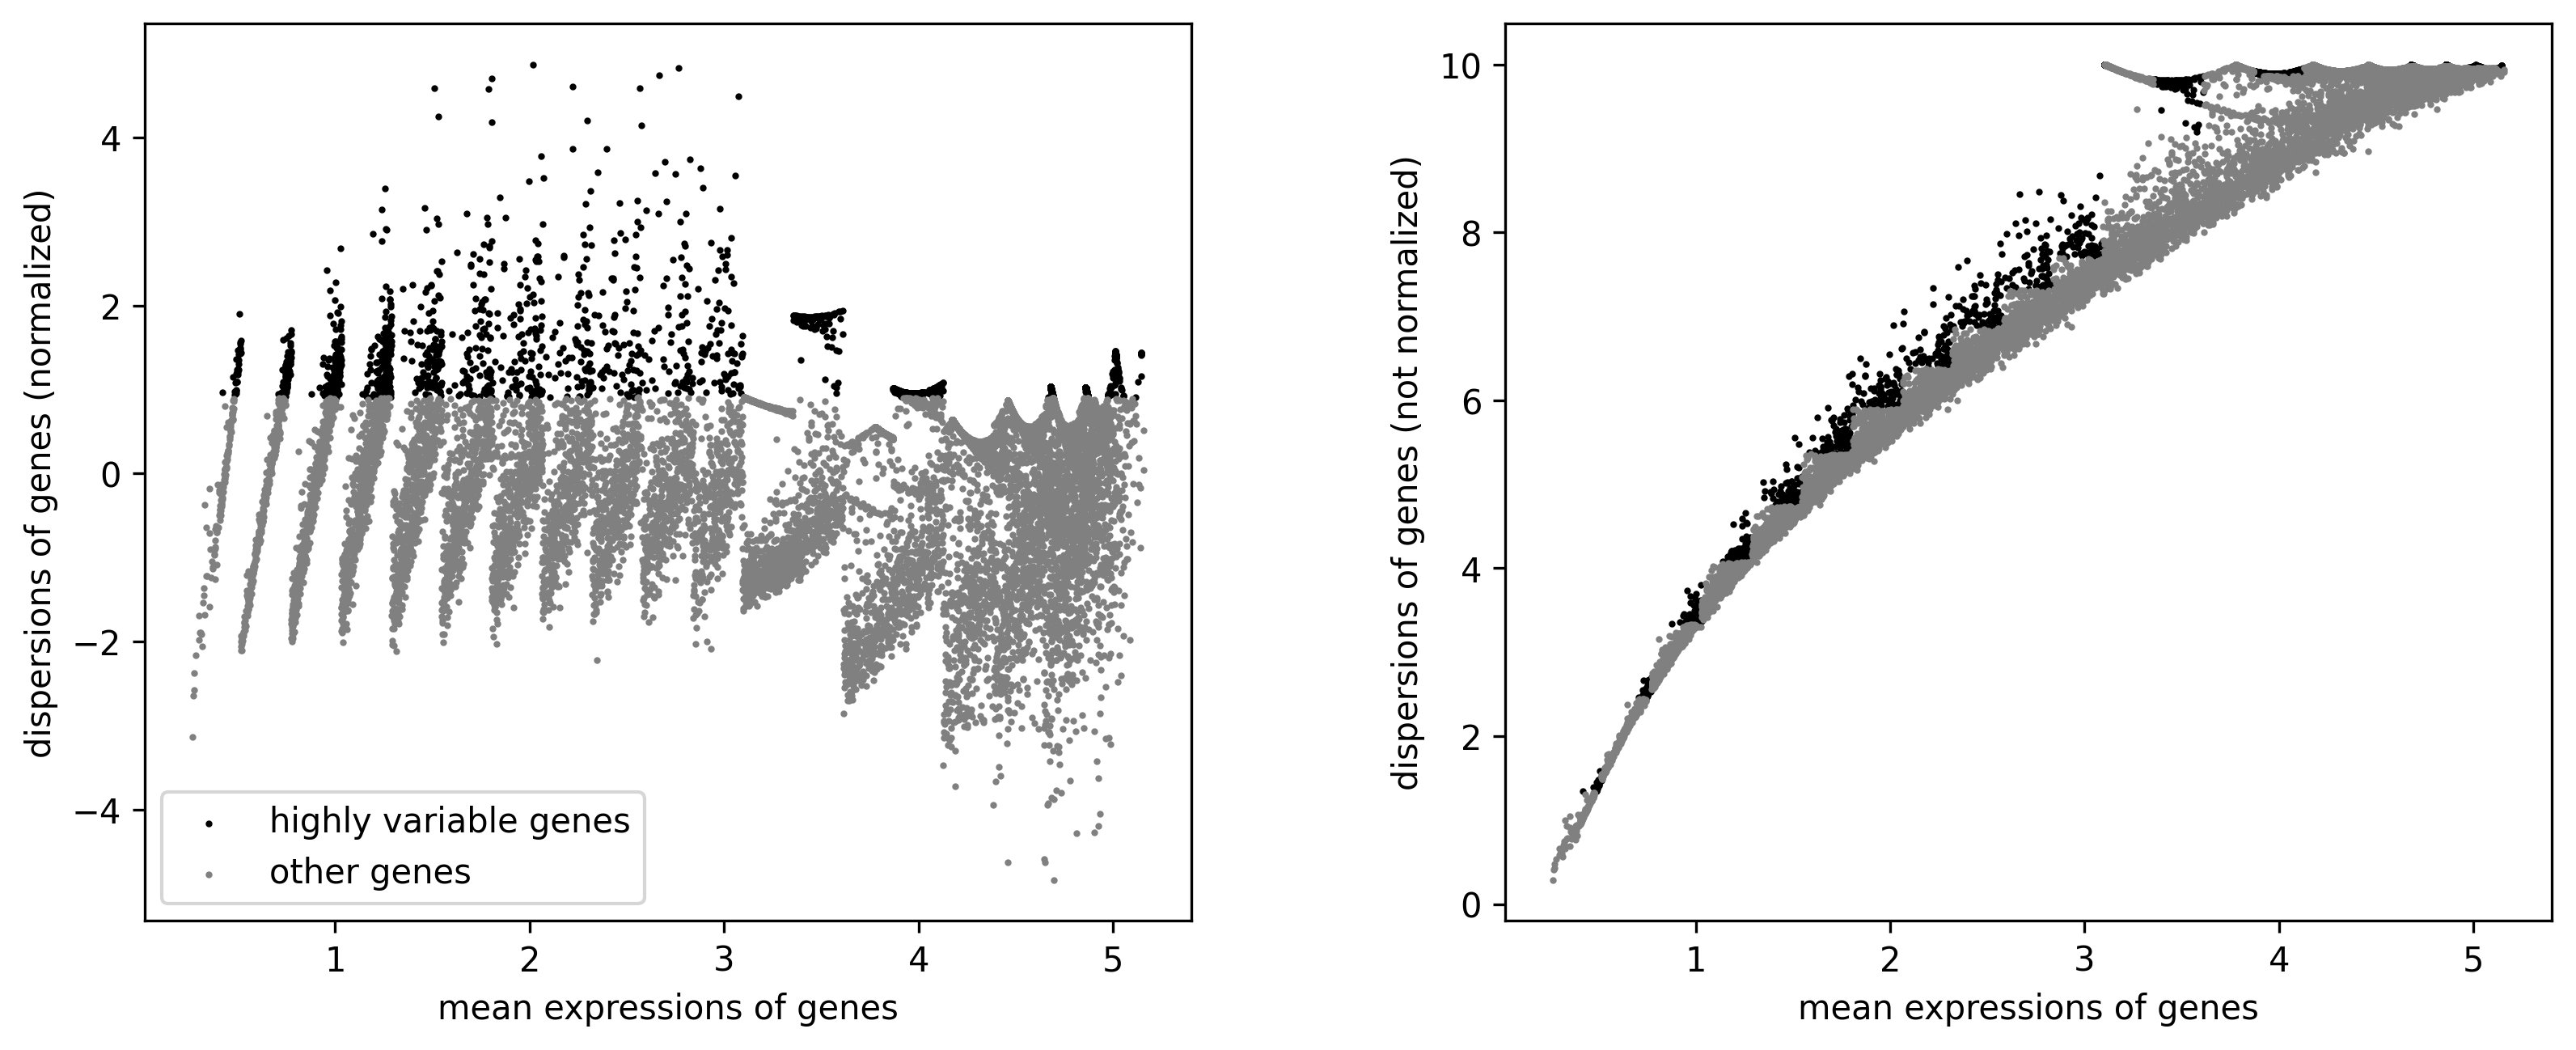
\includegraphics[width=0.8\textwidth]{highly_variable_genes.png}
        \caption{Highly Variable Genes}
        \label{fig:highly_variable_genes}
    \end{figure}
    \newpage

    \begin{figure}[H]
        \centering
        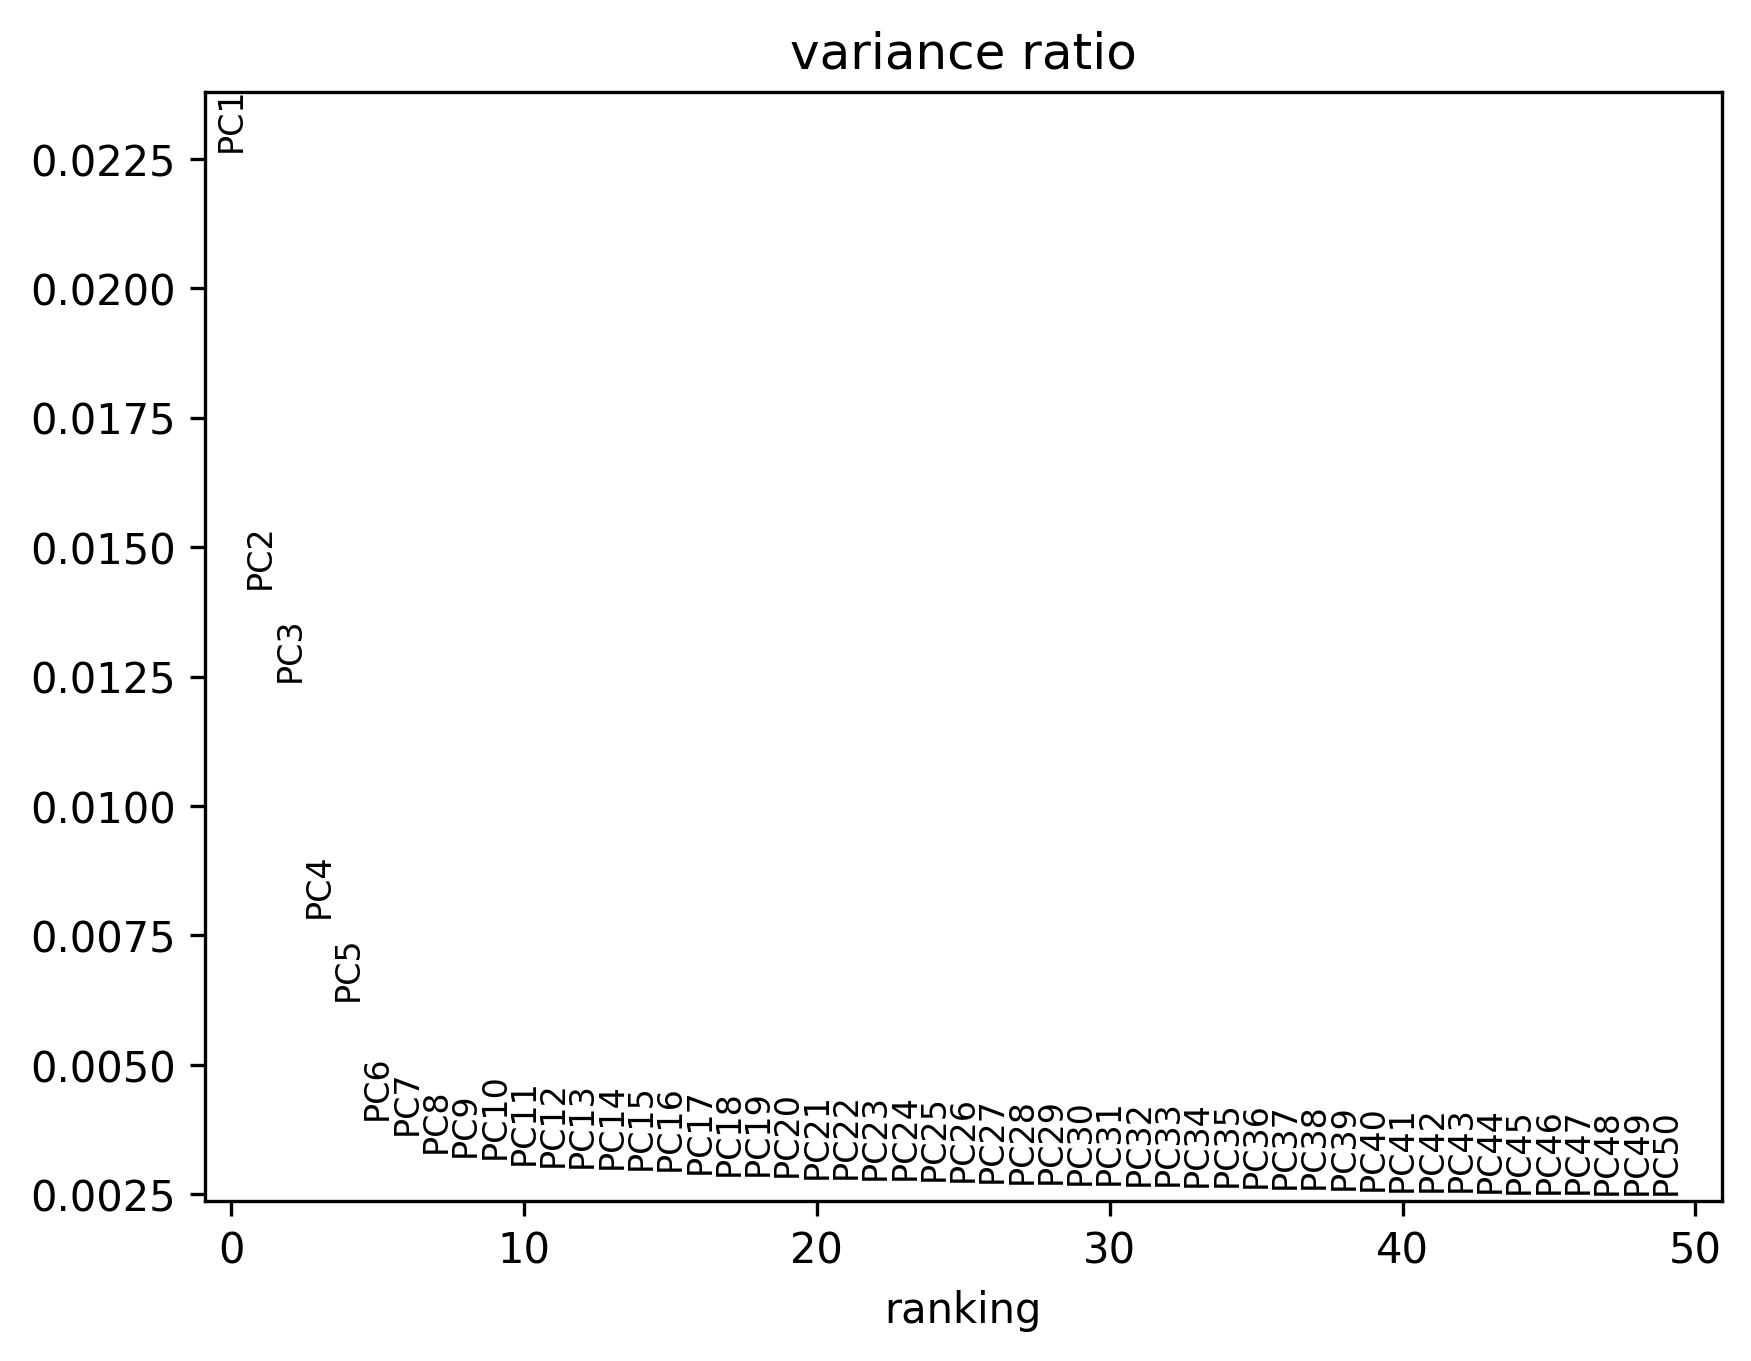
\includegraphics[width=0.8\textwidth]{pca_variance.png}
        \caption{Pca Variance}
        \label{fig:pca_variance}
    \end{figure}
    \newpage

    \begin{figure}[H]
        \centering
        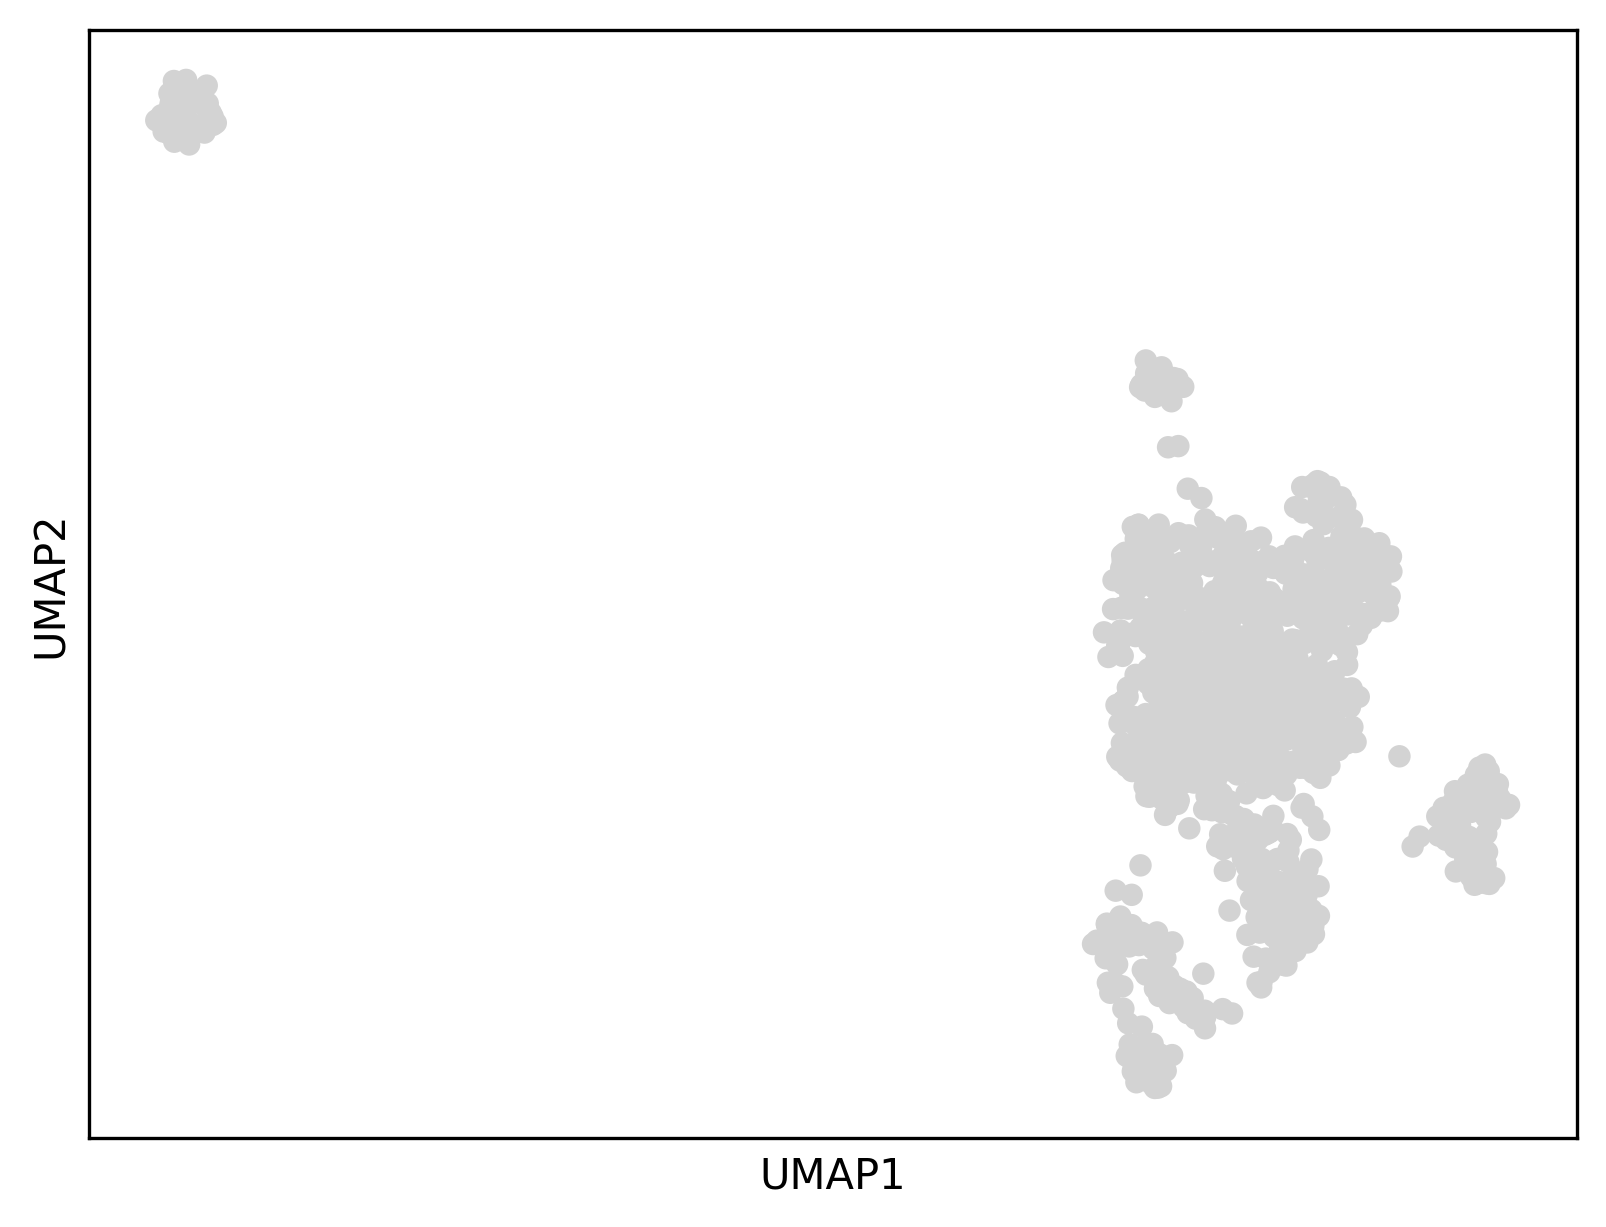
\includegraphics[width=0.8\textwidth]{umap.png}
        \caption{Umap}
        \label{fig:umap}
    \end{figure}
    \newpage

    \begin{figure}[H]
        \centering
        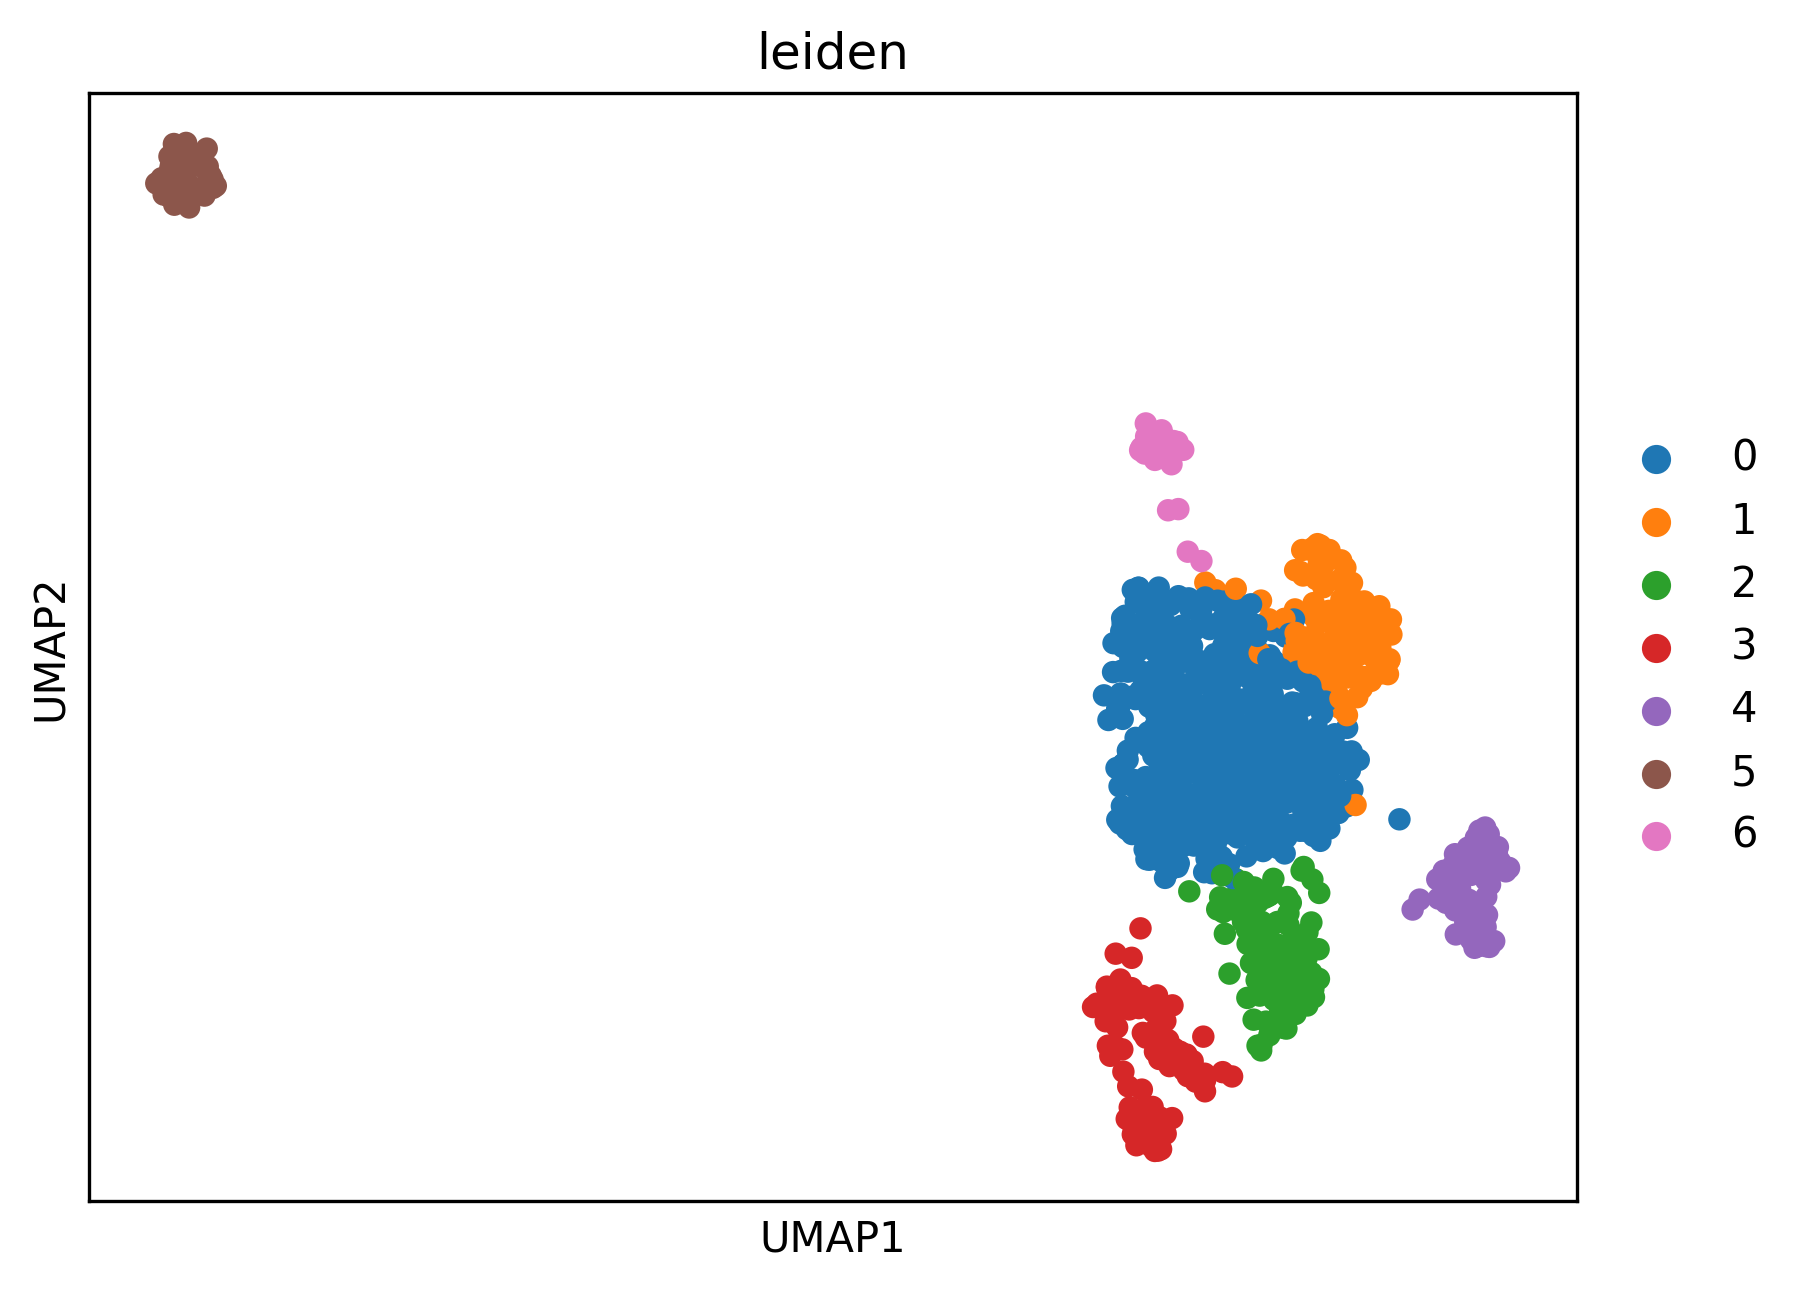
\includegraphics[width=0.8\textwidth]{umap_clusters.png}
        \caption{Umap Clusters}
        \label{fig:umap_clusters}
    \end{figure}
    \newpage

    \begin{figure}[H]
        \centering
        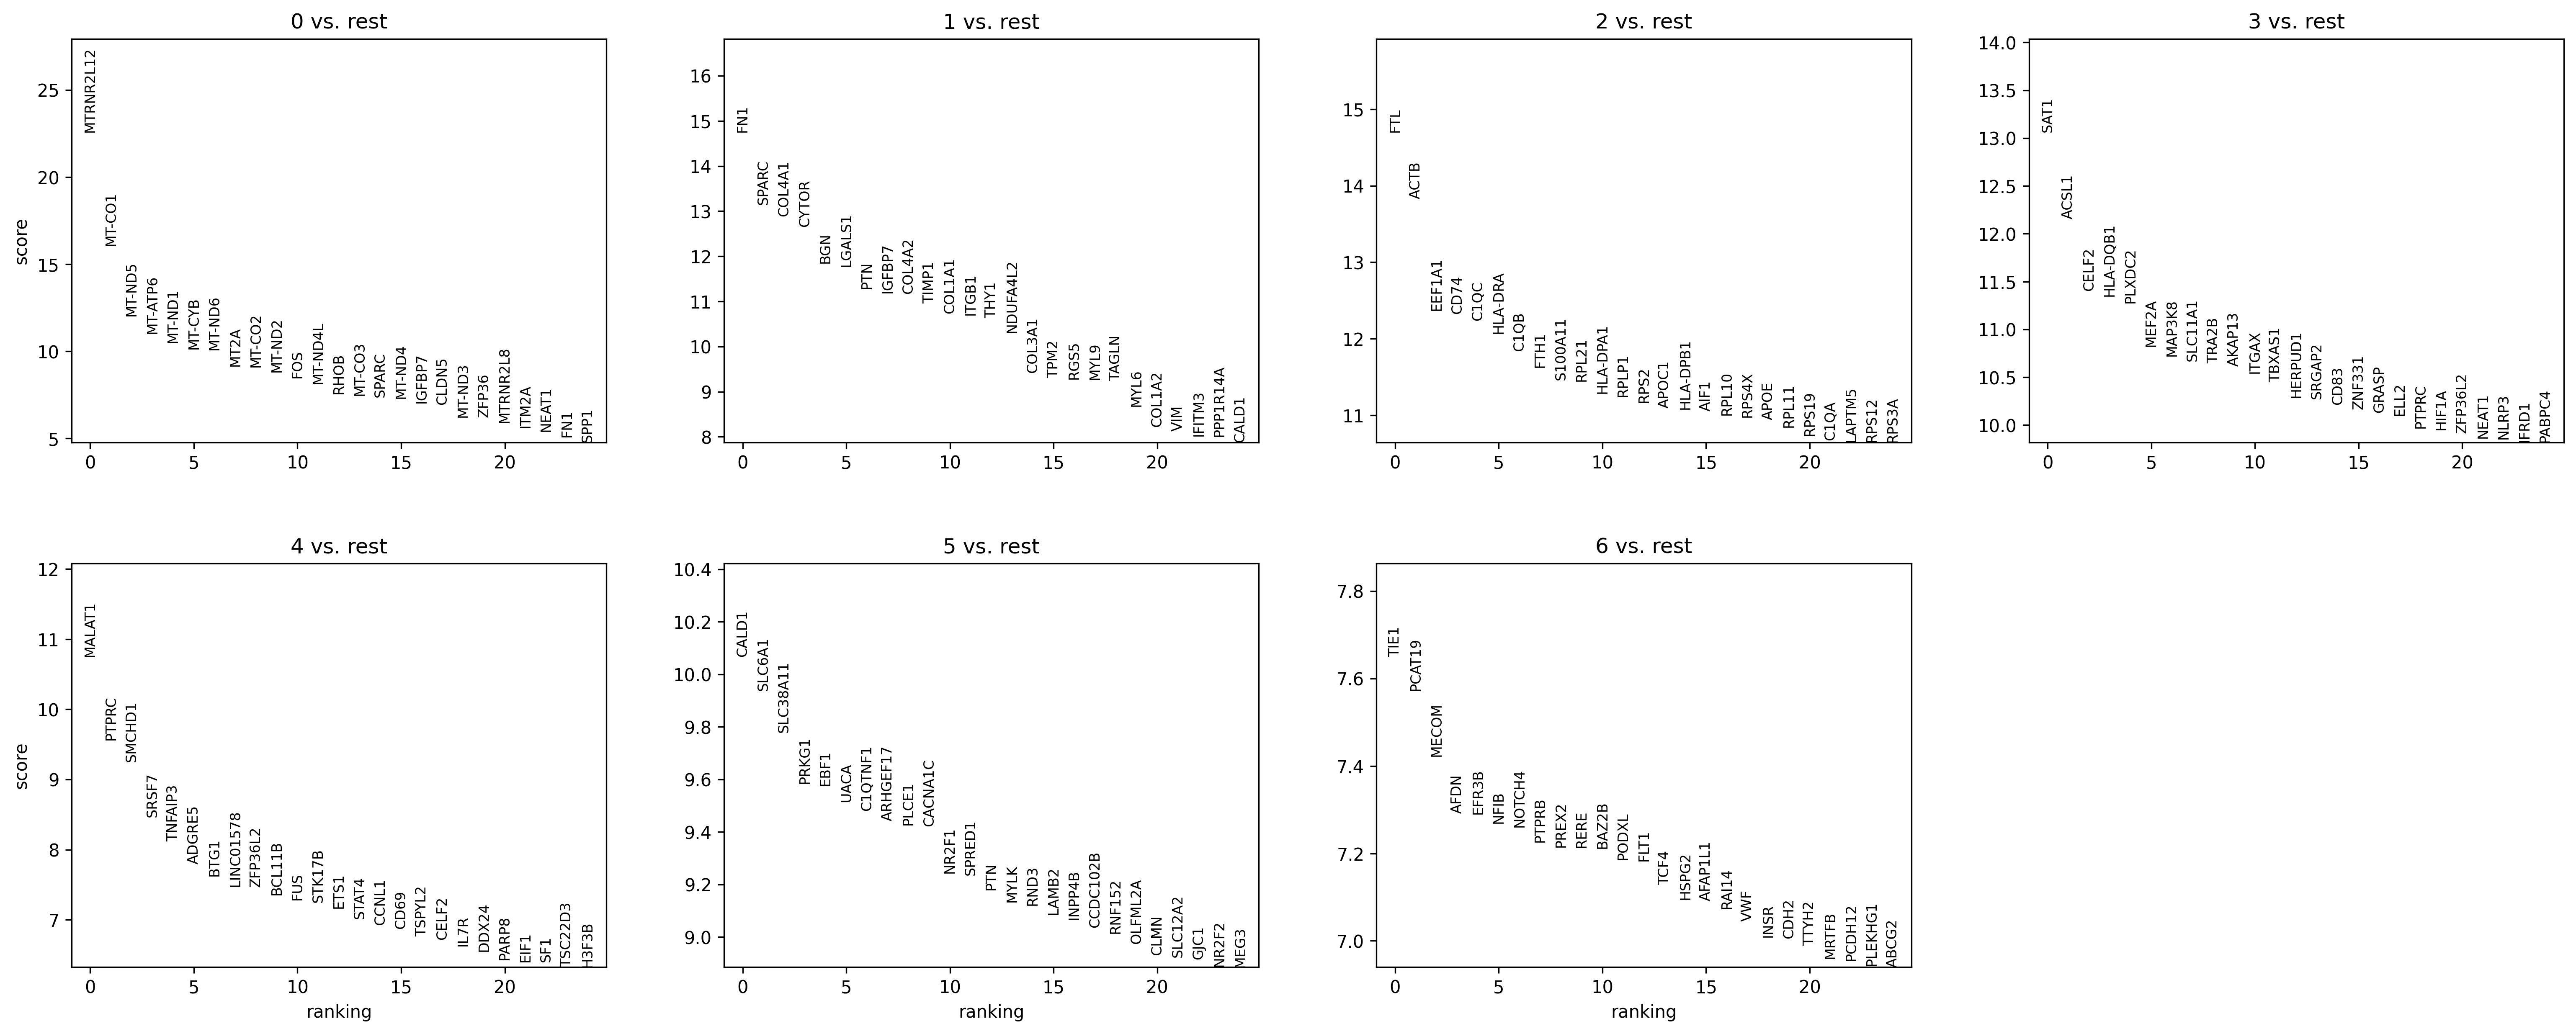
\includegraphics[width=0.8\textwidth]{de.png}
        \caption{De}
        \label{fig:de}
    \end{figure}
    \newpage

\end{document}
